%%%%%%%%%%%%%%%%%%%%%%%%%%%%%%%%%%%%%%%%%%%%%%%%%%%%%%%%%%%%%%%%%%%%
%% I, the copyright holder of this work, release this work into the
%% public domain. This applies worldwide. In some countries this may
%% not be legally possible; if so: I grant anyone the right to use
%% this work for any purpose, without any conditions, unless such
%% conditions are required by law.
%%%%%%%%%%%%%%%%%%%%%%%%%%%%%%%%%%%%%%%%%%%%%%%%%%%%%%%%%%%%%%%%%%%%

\documentclass{beamer}
\usetheme[faculty=ped,basePath=../fibeamer,logo=../fibeamer/logo/mu/Logo-UC-3.png]{fibeamer}
\graphicspath{{../resources/}}

\usepackage{algorithm}
\usepackage{algpseudocode}

\usetheme[faculty=ped]{fibeamer}
\usepackage[utf8]{inputenc}
\usepackage[
  main=english, %% By using `czech` or `slovak` as the main locale
                %% instead of `english`, you can typeset the
                %% presentation in either Czech or Slovak,
                %% respectively.
  czech, slovak %% The additional keys allow foreign texts to be
]{babel}        %% typeset as follows:
%%
%%   \begin{otherlanguage}{czech}   ... \end{otherlanguage}
%%   \begin{otherlanguage}{slovak}  ... \end{otherlanguage}
%%
%% These macros specify information about the presentation
\title{Tuplas y listas} %% that will be typeset on the
\subtitle{Semestre II-2026} %% title page.
\author{Profesora: Andreina Cota Vidaurre}
%% These additional packages are used within the document:
\usepackage{ragged2e}  % `\justifying` text
\usepackage{booktabs}  % Tables
\usepackage{tabularx}
\usepackage{tikz}      % Diagrams
\usetikzlibrary{calc, shapes, backgrounds}
\usetikzlibrary{positioning, arrows.meta, shadows.blur, shapes.geometric}
\usepackage{amsmath, amssymb}
\usepackage{url}       % `\url`s
\usepackage{listings}  % Code listings
\usepackage{graphicx}
\usepackage{amsmath}
\usepackage[T1]{fontenc}
\usepackage{xcolor}
\usepackage{minted}
\usepackage{pifont}
% \usepackage{adjustbox}


% Definicion de pseudocodigo en espaniol
\lstdefinelanguage{PseudocodigoES}{
    morekeywords={INICIO,FIN,PARA,HACER,SI,ENTONCES,FIN_SI,FIN_PARA,IMPRIMIR},
    sensitive=true,
    morecomment=[l]{//},
    morestring=[b]"
}

% Definicion de pseudocodigo en ingles
\lstdefinelanguage{PseudocodeEN}{
    morekeywords={BEGIN,END,FOR,DO,IF,THEN,END_IF,END_FOR,PRINT},
    sensitive=true,
    morecomment=[l]{//},
    morestring=[b]"
}

\lstset{
    basicstyle=\ttfamily\small,
    keywordstyle=\bfseries,
    columns=fullflexible,
    keepspaces=true,
    showstringspaces=false,
    frame=single,
    xleftmargin=0em,
    framexleftmargin=0em,
    framesep=2pt,
    gobble=4,
    resetmargins=true,
    aboveskip=0pt,
    belowskip=0pt
}

\lstdefinestyle{pythonstyle}{
    language=Python,
    basicstyle=\ttfamily\small,
    keywordstyle=\bfseries,
    commentstyle=\itshape,
    stringstyle=\ttfamily,
    showstringspaces=false,
    columns=fullflexible,
    keepspaces=true,
    frame=single,
    breaklines=true,
    xleftmargin=0em,
    framexleftmargin=0em,
    framesep=2pt,
    aboveskip=0pt,
    belowskip=0pt,
    gobble=4,
    resetmargins=true,
    emph={print,input,int,float,str,bool,len,range},
    emphstyle=\bfseries
}

\lstset{style=pythonstyle}

% Estilos del diagrama
\tikzstyle{iniciofin} = [
    ellipse,
    minimum width=2.5cm,
    minimum height=1cm,
    text centered,
    draw=black,
    fill=blue!25
]

\tikzstyle{proceso} = [
    rectangle,
    rounded corners,
    minimum width=3cm,
    minimum height=1cm,
    text centered,
    draw=black,
    fill=cyan!20
]

\tikzstyle{decision} = [
    diamond,
    aspect=2,
    text centered,
    draw=black,
    fill=yellow!35
]

\tikzstyle{flecha} = [
    thick,
    ->,
    >=Stealth
]

% \definecolor{green_python}{HTML}{52A736}

% \newcolumntype{Y}{>{\raggedright\arraybackslash}X}

\frenchspacing
\begin{document}
  \shorthandoff{-}
  \frame[c]{\maketitle}

% \begin{darkframes}

    \begin{frame}{Tuplas y listas}
        \begin{itemize}
            \item Introducción
            \item Lista y Tupla
            \item Lista
            \item Tupla
            \item Índices y Acceso
            \item Funciones y métodos
            \item Ejemplos
            \item Errores comunes
            \item Resumen
        \end{itemize}
    \end{frame}

    \begin{frame}{Introducción}
        \begin{itemize}
            \item Una \textbf{secuencia} es una colección ordenada de elementos.
            \item El orden de la secuencia es importante
            \item Cada elemento ocupa una posición definida y puede ser accedido mediante ella
        \end{itemize}
        Ejemplos cotidianos de secuencia:
        \begin{itemize}
            \item Una fila de personas que espera atención.
            \item Los pasos de una receta de cocina.
            \item Lista de canciones de una playlist.
        \end{itemize}
    \end{frame}

    \begin{frame}{Introducción}
        \begin{itemize}
            \item \textbf{Array} en C, Java y JavaScript.
            \item \textbf{Vector} en C++ y R.
            \item \textbf{Arreglo} en pseudocódigo y en lenguajes como PHP.
            \item \textbf{Lista} en Python, Haskell y Lisp.
        \end{itemize}
    \end{frame}

    \begin{frame}{Características de las secuencias}
        \begin{itemize}
            \item La característica común a todas estas estructuras es el \textbf{acceso por posición (índice)}
            \item El índice se utiliza para indicar en qué lugar de la secuencia se encuentra un elemento
            \item O también para acceder a un elemento en la secuencia
        \end{itemize}
    \end{frame}

    \begin{frame}[fragile,t]{Secuencias en Python}
        \begin{center}
        \begin{tabular}{|l|l|}
        \hline
        \textbf{Tipo} & \textbf{Descripción breve} \\
        \hline
        \mintinline{python}{str}   & Cadena de caracteres (inmutable) \\
        \mintinline{python}{list}  & Lista de elementos (mutable) \\
        \mintinline{python}{tuple} & Tupla de elementos (inmutable) \\
        \mintinline{python}{range} & Secuencia de números generada bajo demanda \\
        \hline
        \end{tabular}
        \end{center}
    \end{frame}

    \begin{frame}[fragile,t]{Lista y Tupla}
        \begin{itemize}
            \item \textbf{Lista} (\mintinline{python}{list}): Colección ordenada, \textbf{mutable} y heterogénea. Se define con corchetes: \mintinline{python}{[ ]}.
            \item \textbf{Tupla} (\mintinline{python}{tuple}): Colección ordenada, \textbf{inmutable} y heterogénea. Se define con paréntesis: \mintinline{python}{( )}.
        \end{itemize}
         
        \begin{center}
        \begin{tabular}{|p{4cm}|p{2.5cm}|p{2.5cm}|}
        \hline
        \textbf{Característica}        & \textbf{Lista}    & \textbf{Tupla} \\
        \hline
        Sintaxis                       & \mintinline{python}{[a, b, c]}  & \mintinline{python}{(a, b, c)} \\
        Mutable (se puede modificar)   & \ding{51}                & No \\
        Permite elementos duplicados   & \ding{51}                & \ding{51} \\
        Permite tipos mixtos           & \ding{51}                & \ding{51} \\
        Uso recomendado                & Datos que cambian & Datos fijos constantes \\
        \hline
        \end{tabular}
        \end{center}
    \end{frame}

    \begin{frame}{Cuándo usar Listas o Tuplas}
        \begin{itemize}
            \item Listas
            \begin{itemize}
                \item Cuando la colección de elementos \textbf{puede cambiar} con el tiempo
                \item Los elementos de la lista pueden agregarse, eliminarse o modificarse
                \item Ejemplos: canciones en una playlist, lista de tareas, participantes inscritos en un curso
            \end{itemize}
            \item Tuplas
            \begin{itemize}
                \item Cuando la colección de elementos \textbf{\ding{55} debe cambiar}
                \item Las tuplas representan un hecho o una constante
                \item Ejemplos: coordenadas GPS de un lugar, fecha de nacimiento, color en formato RGB
            \end{itemize}
        \end{itemize}
        % dibujo de lista y tupla
    \end{frame}

    \begin{frame}{Listas}
        \begin{itemize}
            \item Una lista es una estructura de datos ordenada y mutable que permite almacenar una colección de elementos de cualquier tipo.
            \item Al ser mutable, sus elementos pueden agregarse, modificarse o eliminarse en cualquier momento durante la ejecución del programa.
            \item Se recomienda su uso cuando la colección de datos es dinámica, es decir, cuando se espera que cambie a lo largo del tiempo.
            \item Ejemplos: Lista de compras en el supermercado, lista de tareas, participantes inscritos en un curso.
        \end{itemize}
    \end{frame}

    \begin{frame}{Tuplas}
        \begin{itemize}
            \item Una tupla es una estructura de datos ordenada e inmutable que permite almacenar una colección de elementos de cualquier tipo.
            \item Al ser inmutable, sus elementos no pueden modificarse, agregarse ni eliminarse una vez que la tupla ha sido creada.
            \item Esta característica la hace ideal para representar datos que deben permanecer constantes durante toda la ejecución del programa, garantizando además mayor eficiencia en memoria y tiempo de acceso en comparación con las listas.
            \item Ejemplos: Coordenadas de un campus \texttt{(-33.4980, -70.6150, 560)}, registro de un estudiante \texttt{("Ana Pérez", 20234567, "IP")}, fecha y hora de una evaluación \texttt{(2026, 6, 15, 9, 30)}.
        \end{itemize}
    \end{frame}

    \begin{frame}[fragile, t]{Índices y acceso}
        \begin{itemize}
            \item El \textbf{índice} es la posición de un elemento en una secuencia. En Python, los índices comienzan en \textbf{0}.
            \begin{minted}[xleftmargin=-2cm, frame=leftline, fontsize=\small]{python} 
            cursos = ["IP", "Cálculo", "Álgebra", "Física"]
            #índices:   0        1          2          3
            print(cursos[0])   # IP
            print(cursos[2])   # Álgebra
            \end{minted}
            \item Los índices negativos permiten contar desde el \textbf{final} de la secuencia.
            \begin{minted}[xleftmargin=-2cm, frame=leftline, fontsize=\small]{python}
            cursos = ["IP", "Cálculo", "Álgebra", "Física"]
            #índices:  -4       -3         -2         -1
            print(cursos[-1])   # Física
            print(cursos[-2])   # Álgebra
            \end{minted}
        \end{itemize}
    \end{frame}

    \begin{frame}[fragile, t]{Funciones: Slicing (rebanado)}
        El slicing permite obtener una subsecuencia mediante la sintaxis \texttt{[inicio:fin:paso]}, donde \texttt{fin} es \textbf{exclusivo}.

        \begin{minted}[xleftmargin=-2cm, frame=leftline, fontsize=\small]{python}
            datos = ["Python", "Git", 1.0, True, 39]
 
            print(datos[1:4])    # ['Git', 1.0, True]
            print(datos[:3])     # ['Python', 'Git', 1.0]
            print(datos[::2])    # ['Python', 1.0, 39]
            print(datos[::-1])   # [39, True, 1.0, 'Git', 'Python']
        \end{minted}
    \end{frame}

    \begin{frame}[fragile, t]{Funciones: Modificar una Tupla}
        Intentar modificar un elemento de una tupla genera un error en tiempo de ejecución:

        \begin{minted}[xleftmargin=-2cm, frame=leftline, fontsize=\small]{python}
            coordenadas = (-33.4500, -70.6600, 560)
            coordenadas[0] = -33.9000   
            # TypeError: 'tuple' object does not support item assignment
        \end{minted}
        Este comportamiento es \textbf{intencional}: garantiza que los datos inmutables no se alteren por error durante la ejecución del programa.
    \end{frame}

    \begin{frame}[fragile,t]{Funciones de listas y tuplas}
        \begin{center}
        \begin{tabular}{|p{2cm}|p{0.6cm}|p{0.6cm}|p{5.8cm}|}
        \hline
        \textbf{Operación / Método} & \textbf{Lista} & \textbf{Tupla} & \textbf{Descripción} \\
        \hline
        \mintinline{python}{len(x)}         & \ding{51} & \ding{51} & Cantidad de elementos \\
        \mintinline{python}{x.count(v)}     & \ding{51} & \ding{51} & Cuántas veces aparece \texttt{v} \\
        \mintinline{python}{x.index(v)}     & \ding{51} & \ding{51} & Índice de la primera ocurrencia de \texttt{v} \\
        \mintinline{python}{v in x}         & \ding{51} & \ding{51} & Verifica si \texttt{v} pertenece a \texttt{x} \\
        \mintinline{python}{x + y}          & \ding{51} & \ding{51} & Concatenación de dos secuencias \\
        \mintinline{python}{x * n}          & \ding{51} & \ding{51} & Repetición \texttt{n} veces \\
        \hline
        \end{tabular}
        \end{center}
    \end{frame}

    \begin{frame}[fragile,t]{Funciones de listas y tuplas}
        \begin{center}
        \begin{tabular}{|p{2.5cm}|p{0.6cm}|p{0.6cm}|p{5.3cm}|}
        \hline
        \textbf{Operación / Método} & \textbf{Lista} & \textbf{Tupla} & \textbf{Descripción} \\
        \hline
        \mintinline{python}{x.append(v)}    & \ding{51} & \ding{55} & Agrega \texttt{v} al final \\
        \mintinline{python}{x.insert(i, v)} & \ding{51} & \ding{55} & Inserta \texttt{v} en la posición \texttt{i} \\
        \mintinline{python}{x.remove(v)}    & \ding{51} & \ding{55} & Elimina la primera ocurrencia de \texttt{v} \\
        \mintinline{python}{x.pop(i)}       & \ding{51} & \ding{55} & Elimina y retorna el elemento en posición \texttt{i} \\
        \mintinline{python}{x.sort()}       & \ding{51} & \ding{55} & Ordena la lista en sitio \\
        \mintinline{python}{x.reverse()}    & \ding{51} & \ding{55} & Invierte la lista en sitio \\
        \mintinline{python}{x.clear()}      & \ding{51} & \ding{55} & Elimina todos los elementos \\
        \hline
        \end{tabular}
        \end{center}
    \end{frame}

    \begin{frame}[fragile, t]{Ejemplos de uso: \mintinline{python}{list}}
        \begin{itemize}
            \item Inicializar una lista
            \begin{minted}[xleftmargin=-2cm, frame=leftline, fontsize=\small]{python}
            estudiantes = ["Ana", "Luis", "María", "Pedro"]
            \end{minted}
            \item Tamaño de la lista
            \begin{minted}[xleftmargin=-2cm, frame=leftline, fontsize=\small]{python}
            print(len(estudiantes))          # 4
            \end{minted}
            \item Verificar existencia de un elemento
            \begin{minted}[xleftmargin=-2cm, frame=leftline, fontsize=\small]{python}
            print("Luis" in estudiantes) # True
            \end{minted}
            \item Agregar elemento
            \begin{minted}[xleftmargin=-2cm, frame=leftline, fontsize=\small]{python}
            estudiantes.append("Carla")
            print(estudiantes)
            # ["Ana", "Luis", "María", "Pedro", "Carla"]
            \end{minted}
        \end{itemize}
    \end{frame}

    \begin{frame}[fragile, t]{Ejemplos de uso: \mintinline{python}{list}}
        \begin{itemize}
            \item Eliminar un elemento
            \begin{minted}[xleftmargin=-2cm, frame=leftline, fontsize=\small]{python}
            estudiantes.remove("Luis")
            print(estudiantes)
            # ['Ana', 'María', 'Pedro', "Carla"]
            \end{minted}
            \item Insertar elemento en una posición específica
            \begin{minted}[xleftmargin=-2cm, frame=leftline, fontsize=\small]{python}
            estudiantes.insert(1, "Diego")
            print(estudiantes)
            # ['Ana', 'Diego', 'María', 'Pedro', "Carla"]
            \end{minted}
            \item Contar elementos que cumplen una condición
            \begin{minted}[xleftmargin=-2cm, frame=leftline, fontsize=\small]{python}
            con_a = [p for p in estudiantes if "a" in p.lower()]
            print(f"Nombres con 'a': {len(con_a)}")
            # Nombres con 'a': 3
            \end{minted}
        \end{itemize}
    \end{frame}

    \begin{frame}[fragile, t]{Ejemplos de uso:\mintinline{python}{tuple}}
        \begin{itemize}
            \item Inicializar una tupla
            \begin{minted}[xleftmargin=-2cm, frame=leftline, fontsize=\small]{python}
            campus = ("San Joaquín", -33.4980, -70.6150, 560)
            \end{minted}
            \item Tamaño de la tupla
            \begin{minted}[xleftmargin=-2cm, frame=leftline, fontsize=\small]{python} 
            print(len(campus))          # 4
            \end{minted}
            \item Posición de la primera ocurrencia de un valor
            \begin{minted}[xleftmargin=-2cm, frame=leftline, fontsize=\small]{python}
            print(campus.index(-33.4980))  # 1
            \end{minted}
            \item Verificar existencia de un elemento
            \begin{minted}[xleftmargin=-2cm, frame=leftline, fontsize=\small]{python}
            print(560 in campus)
            # True
            \end{minted}
        \end{itemize}
    \end{frame}

    \begin{frame}[fragile,t]{Similitud con Strings}
        El tipo \texttt{str} en Python es también una secuencia, lo que significa que comparte comportamientos fundamentales con \texttt{list} y \texttt{tuple}.
        \begin{center}
        \begin{tabular}{|l|c|c|c|}
        \hline
        \textbf{Operación}         & \textbf{str} & \textbf{list} & \textbf{tuple} \\
        \hline
        Acceso por índice          & \ding{51} & \ding{51} & \ding{51} \\
        Índices negativos          & \ding{51} & \ding{51} & \ding{51} \\
        Slicing                    & \ding{51} & \ding{51} & \ding{51} \\
        \texttt{len()}             & \ding{51} & \ding{51} & \ding{51} \\
        \texttt{in} / \texttt{not in} & \ding{51} & \ding{51} & \ding{51} \\
        Iteración con \texttt{for} & \ding{51} & \ding{51} & \ding{51} \\
        Concatenación \texttt{+}   & \ding{51} & \ding{51} & \ding{51} \\
        Repetición \texttt{*}      & \ding{51} & \ding{51} & \ding{51} \\
        Mutable                    & \ding{55} & \ding{51} & \ding{55} \\
        \hline
        \end{tabular}
        \end{center}
    \end{frame}

    \begin{frame}[fragile,t]{Diferencias de listas y tuplas con strings}
        \begin{itemize}
            \item Un \mintinline{python}{str} solo contiene \textbf{caracteres}.
            \item Una \mintinline{python}{list} o \mintinline{python}{tuple} puede contener \textbf{cualquier tipo de dato}: números, cadenas, booleanos, otras listas, etc.
            \item Tanto \mintinline{python}{str} como \mintinline{python}{tuple} son \textbf{inmutables}: una vez creados, sus elementos no pueden modificarse directamente.
        \end{itemize}
    \end{frame}

    \begin{frame}[fragile, t]{Ejemplos comparativos}
        \begin{minted}[xleftmargin=-2cm, frame=leftline, fontsize=\small]{python}
            curso   = "NOTAS"               # str
            letras  = ["N","O","T","A","S"]  # list
            clave   = ("N","O","T","A","S")  # tuple
             
            print(curso[0])    # N
            print(letras[0])   # N
            print(clave[0])    # N
        \end{minted}
    \end{frame}

    \begin{frame}[fragile, t]{Ejercicio 1: Registro de un grupo}
        Se tiene una lista con los integrantes de un grupo de trabajo. Realice las siguientes operaciones:
        \begin{enumerate}
            \item Agregar un nuevo integrante
            \item Eliminar a quien se retiró del curso
            \item Mostrar al coordinador del grupo (primer elemento)
            \item Mostrar el tamaño final del grupo
        \end{enumerate}
        \begin{minted}[xleftmargin=-2cm, frame=leftline, fontsize=\small]{python}
            grupo = ["Ana Pérez", "Luis López", "María Rivas", \
            "Pedro Mora", "Carla Díaz"]
            # Agregar integrante
            grupo.append("Diego Fuentes")
        \end{minted}
    \end{frame}

    \begin{frame}[fragile, t]{Ejercicio 1: Registro de un grupo}
        \begin{minted}[xleftmargin=-2cm, frame=leftline, fontsize=\small]{python}
            # Eliminar a quien se retiró
            grupo.remove("María Rivas")
             
            # Mostrar coordinador del grupo
            print(f"Coordinador: {grupo[0]}")
            # Coordinador: Ana Pérez
             
            # Mostrar tamaño del grupo
            print(f"Integrantes actuales: {len(grupo)} estudiantes")
            # Integrantes actuales: 5 estudiantes
             
            print(grupo)
            # ['Ana Pérez', 'Luis López', 'Pedro Mora',
            #  'Carla Díaz', 'Diego Fuentes']
        \end{minted}
    \end{frame}

    \begin{frame}[fragile, t]{Ejercicio 2: Coordenadas de campus}
        Se registran tres sedes universitarias como tuplas. Se pide:
        \begin{enumerate}
            \item Almacenarlas en una lista de campus
            \item Mostrar la cantidad total de sedes
            \item Acceder a las coordenadas del segundo campus
        \end{enumerate}
        \begin{minted}[xleftmargin=-2cm, frame=leftline, fontsize=\small]{python}
            # Solución
            campus_1 = ("San Joaquín",  -33.4980, -70.6150)
            campus_2 = ("Casa Central", -33.4410, -70.6400)
            campus_3 = ("Oriente",      -33.4400, -70.5800)

            # Lista de campus (lista de tuplas)
            campus = [campus_1, campus_2, campus_3]
        \end{minted}
    \end{frame}

    \begin{frame}[fragile, t]{Ejercicio 2: Coordenadas de campus}
        \begin{minted}[xleftmargin=-2cm, frame=leftline, fontsize=\small]{python}
            print(f"Total de sedes: {len(campus)}")
            # Total de sedes: 3
             
            # Acceder al segundo campus
            print(f"Segundo campus : {campus[1][0]}")
            # Segundo campus : Casa Central
             
            print(f"Latitud        : {campus[1][1]}")
            # Latitud        : -33.441
             
            print(f"Longitud       : {campus[1][2]}")
            # Longitud       : -70.64
        \end{minted}
    \end{frame}

    \begin{frame}[fragile, t]{Errores comunes y cómo interpretarlos}
        \begin{center}
        \begin{tabular}{|l|p{3.5cm}|p{3.5cm}|}
        \hline
        \textbf{Error} & \textbf{Causa} & \textbf{Solución} \\
        \hline
        \mintinline{python}{IndexError} & Índice fuera del rango de la secuencia &
            Verificar \mintinline{python}{len()} antes de acceder \\
        \mintinline{python}{TypeError} & Intentar modificar una tupla o un string &
            Usar lista si se requiere mutabilidad \\
        \mintinline{python}{ValueError} & \mintinline{python}{.remove()} o \mintinline{python}{.index()} con un valor inexistente &
            Usar \mintinline{python}{in} para verificar antes \\
        \hline
        \end{tabular}
        \end{center}
    \end{frame}

    \begin{frame}[fragile, t]{Errores comunes y cómo interpretarlos}
        \begin{minted}[xleftmargin=-2cm, frame=leftline, fontsize=\small]{python}
            # IndexError
            cursos = ["IP", "Cálculo", "Física"]
            print(cursos[5])       
            # IndexError: list index out of range
             
            # TypeError
            coord = (10.0, 20.0)
            coord[0] = 15.0        
            # TypeError: 'tuple' object does not support item assignment
             
            # ValueError
            materias = ["Álgebra", "Química"]
            materias.remove("Historia") 
            # ValueError: list.remove(x): x not in list
        \end{minted}
    \end{frame}

    \begin{frame}{Lista vs Tupla}
        \begin{figure}
            \centering
            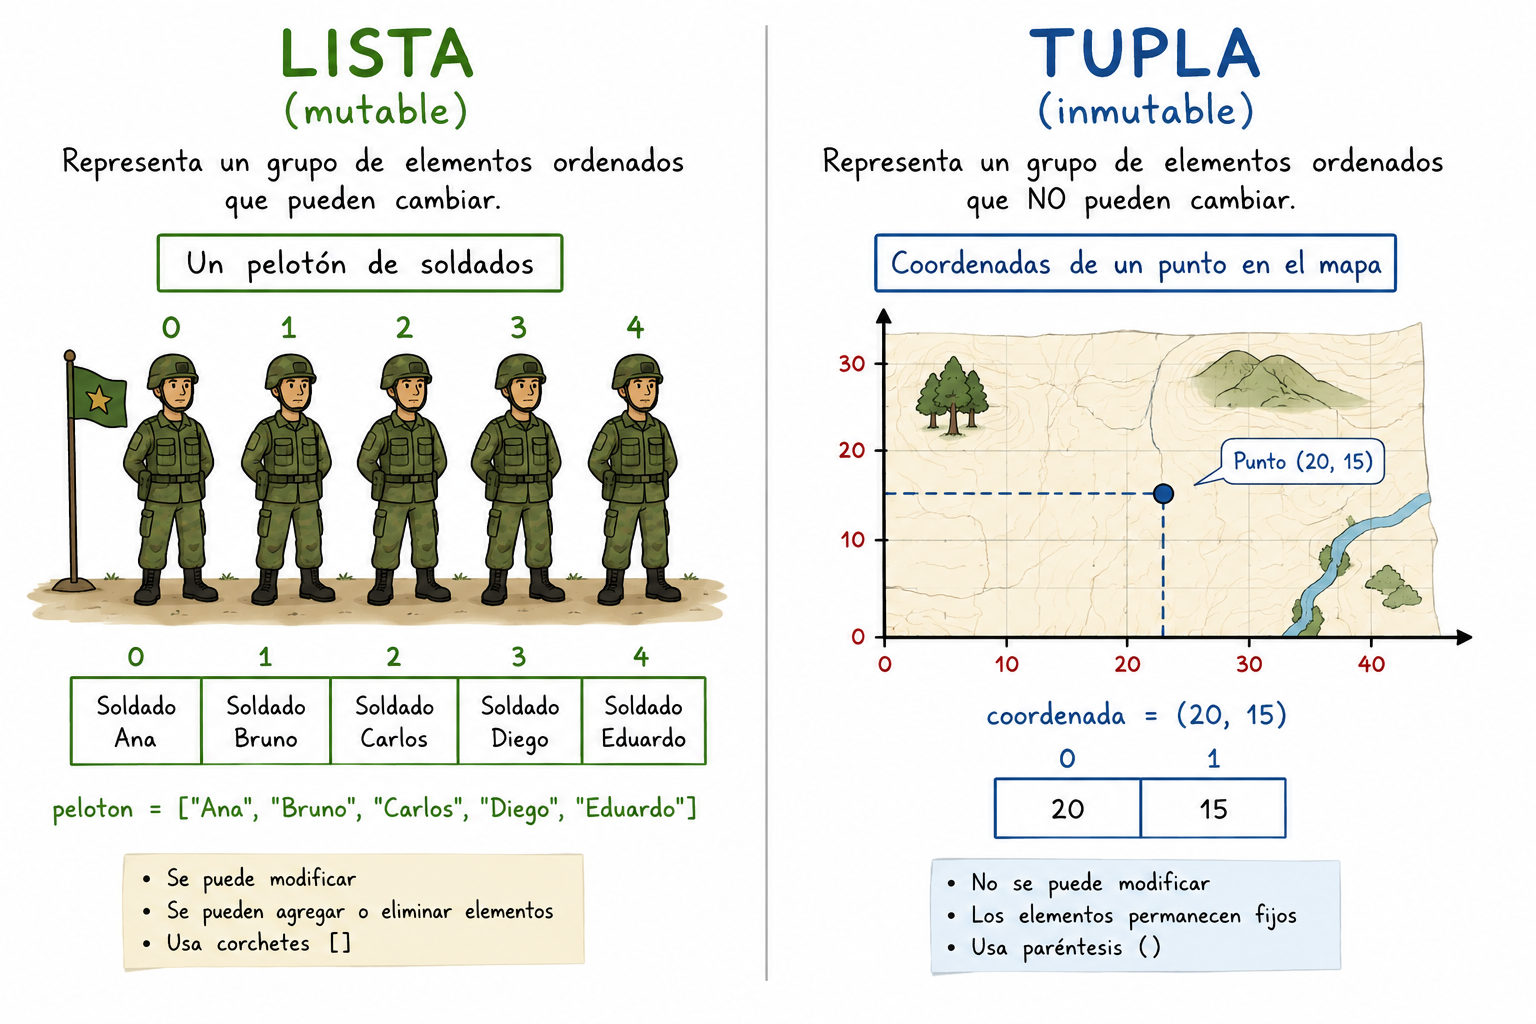
\includegraphics[width=\linewidth]{lista_tupla.png}
        \end{figure}
    \end{frame}

    \begin{frame}[fragile,t]{\mintinline{python}{list, tuple}}
        \begin{itemize}
            \item Listas
            \begin{itemize}
                \item Colección ordenada y \textbf{mutable}: sus elementos pueden agregarse, modificarse o eliminarse.
                \item Se definen con corchetes: \mintinline{python}{['a', 1, 'b', 3.0, True]}
                \item Usar cuando los datos \textbf{cambian} en el tiempo
                \item Métodos exclusivos: \mintinline{python}{append(), remove(), insert(), sort(), pop()}
            \end{itemize}
            \item Tuplas
            \begin{itemize}
                \item Colección ordenada e \textbf{inmutable}: una vez creada, no puede modificarse.
                \item Se definen con paréntesis: \mintinline{python}{('a', 1, 'b', 3.0, True)}
                \item Usar cuando los datos deben permanecer \textbf{constantes}
                \item Intentar modificarlas genera un \mintinline{python}{TypeError}
            \end{itemize}
        \end{itemize}
    \end{frame}

    \begin{frame}[fragile,t]{\mintinline{python}{list, tuple}}
        \begin{itemize}
            \item Lo que comparten
            \begin{itemize}
                \item Acceso por índice positivo y negativo
                \item Slicing \mintinline{python}{[inicio:fin:paso]}
                \item Funciones: \mintinline{python}{len(), count(), index()}, operador \mintinline{python}{in}
                \item Ambas son secuencias, al igual que \mintinline{python}{str}: misma lógica de acceso e iteración
            \end{itemize}
            \item Regla de oro
            \begin{itemize}
                \item ¿Los datos cambian? $\rightarrow$ Lista
                \item ¿Los datos son fijos? $\rightarrow$ Tupla
            \end{itemize}
        \end{itemize}
    \end{frame}
    
\end{document}
